\documentclass[../main.tex]{subfiles}
\graphicspath{{figures/}{../figures/}}

\begin{document}
% \todo[color=green!40]{完成问题三模型的求解(sections/q3\_solution)}

由于问题5的变量较多,直接使用启发式搜索算法进行优化非常容易陷入局部最优解中,并且与实际最优解差距过大。因此,我们采用的优化策略是先逐个优化一个无人机对三个导弹的投放策略,再将得到的有效时间合并(去掉重复有效时间)。反复操作,得到多组不同的投放策略和有效时间,再对比这些投放策略,选取其中有效时间最长的一组作为最优投放策略。以下是核心步骤:

\textbf{步骤1 系统初始化}
\begin{itemize}
    \item 设置初始参数:无人机飞行方向角、飞行速度速度、烟幕弹投放和起爆时间;
    \item 计算投放点与起爆点;
    \item 逐个离散时刻判断:计算导弹位置、判断烟幕是否完全遮蔽,若完全遮蔽则有效,反之,无效;
    \item 。
\end{itemize}

\textbf{步骤2 无人机独立优化}
\begin{itemize}
    \item 优化变量:方向角、速度、投放增量、延迟时间,设边界;
    \item 多轮差分优化:每架优化5次,目标最大总遮蔽时间;
    \item 转换最优变量为参数,计算单架无人机对各个导弹的贡献(单独激活1架,其余参数无效)献;
\end{itemize}

合并5架最优参数,重新评估整体效果。

\textbf{步骤4 结果输出}
\begin{itemize}
    \item 合并效果:总遮蔽时间、单导弹遮蔽时间与区间;
    \item 单架无人机投放策略:飞行方向、飞行速度、投放/起爆位置、贡献值。
\end{itemize}






\begin{table}[H]
\caption{问题5投放策略-1}
\label{tab:001} 
\centering
\begin{small}
\begin{tabular}{cccc}
\toprule[1.5pt]
无人机编号 &无人机运动方向 & 无人机运动速度  &烟幕干扰弹编号     \\  
\midrule[1pt]
  FY1           &7.45                   & 72.00     & 1     \\               
   FY1          &7.45                  & 72.00     & 2      \\               
   FY1          &7.45                   & 72.00     & 3    \\                
  FY2           &295.07                   & 127.02     & 1      \\                
  FY2           &295.07                   & 127.02     & 2       \\               
  FY2           &295.07                   & 127.02    & 3     \\               
  FY3           & 79.64                  & 82.34     & 1       \\               
FY3             & 79.64                  & 82.34     & 2    \\                
FY3             & 79.64                  & 82.34    & 3      \\                
  FY4           &0                   & 70.00     & 1      \\                
  FY4           &0                   & 70.00     & 2       \\               
  FY4           &0                   & 70.00    & 3     \\               
  FY5          & 120.32                 & 104.78     & 1       \\               
FY5         & 120.32                 & 104.78    & 2    \\                
FY5          &120.32                  & 104.78     & 3      \\               
\bottomrule[1.5pt]
\end{tabular}
\end{small}
\end{table}


\begin{table}[H]
\caption{问题5投放策略-2}
\label{tab:031} 
\centering
\begin{small}
\begin{tabular}{cccc}
\toprule[1.5pt]
烟幕干扰弹投放点的x坐标& 烟幕干扰弹投放点的y坐标    &烟幕干扰弹投放点的z坐标 & 烟幕干扰弹起爆点的x坐标\\
\midrule[1pt]
    17800.71 & 0.09    & 1800.00 & 17801.43 \\
    17871.39 & 9.33    & 1800.00 & 17903.52 \\
    19121.47 & 172.77  & 1800.00 & 19180.73 \\
    12425.24 & 491.10  & 1400.00 & 12457.54 \\
    12707.30 & -111.76 & 1400.00 & 12851.56 \\
    13363.47 & -1514.23& 1400.00 & 13757.49 \\
    6501.92  & -254.17 & 700.00  & 6509.32 \\
    6516.87  & -172.36 & 700.00  & 6555.07 \\
    6531.68  & -91.36  & 700.00  & 6564.69 \\
    11064.40 & 2000.00 & 1800.00 & 11099.40 \\
    11134.40 & 2000.00 & 1800.00 & 11228.20 \\
    11204.40 & 2000.00 & 1800.00 & 11239.40 \\
    12151.52 & -549.23 & 1300.00 & 11821.44 \\
    12069.53 & -409.04 & 1300.00 & 11821.4 \\
    11858.99 & -49.06  & 1300.00 & 11759.02 \\
\bottomrule[1.5pt]
\end{tabular}
\end{small}
\end{table}




\begin{table}[H]
\caption{问题5投放策略-3}
\label{tab:031} 
\centering
\begin{small}
\begin{tabular}{cccc}
\toprule[1.5pt]
干扰弹起爆点的y坐标&干扰弹起爆点的z坐标&有效干扰时长 &干扰的导弹编号\\
\midrule[1pt]
0.19    & 1800.00 & 2.64 & M1 \\
    13.53   & 1799.01 & 4.50 & M1 \\
    180.51  & 1796.62 & 0    & 0 \\
    422.07  & 1398.24 & 4.09 & M2 \\
    -420.10 & 1364.81 & 3.38 & M3 \\
    -2356.40& 1137.45 & 0    & 0 \\
    -213.67 & 698.77  & 1.57 & M3 \\
    36.61   & 667.38  & 2.90 & M1 \\
    89.26   & 675.63  & 0    & 0 \\
    2000.00 & 1798.78 & 0    & 0 \\
    2000.00 & 1791.20 & 0    & 0 \\
    2000.00 & 1798.78 & 0    & 0 \\
    -399.99 & 1286.66 & 1.04 & M3 \\
    15.16   & 1192.22 & 3.51 & M1 \\
    121.89  & 1282.50 & 0    & 0 \\             
\bottomrule[1.5pt]
\end{tabular}
\end{small}
\end{table}
\begin{figure}[H]
\centering
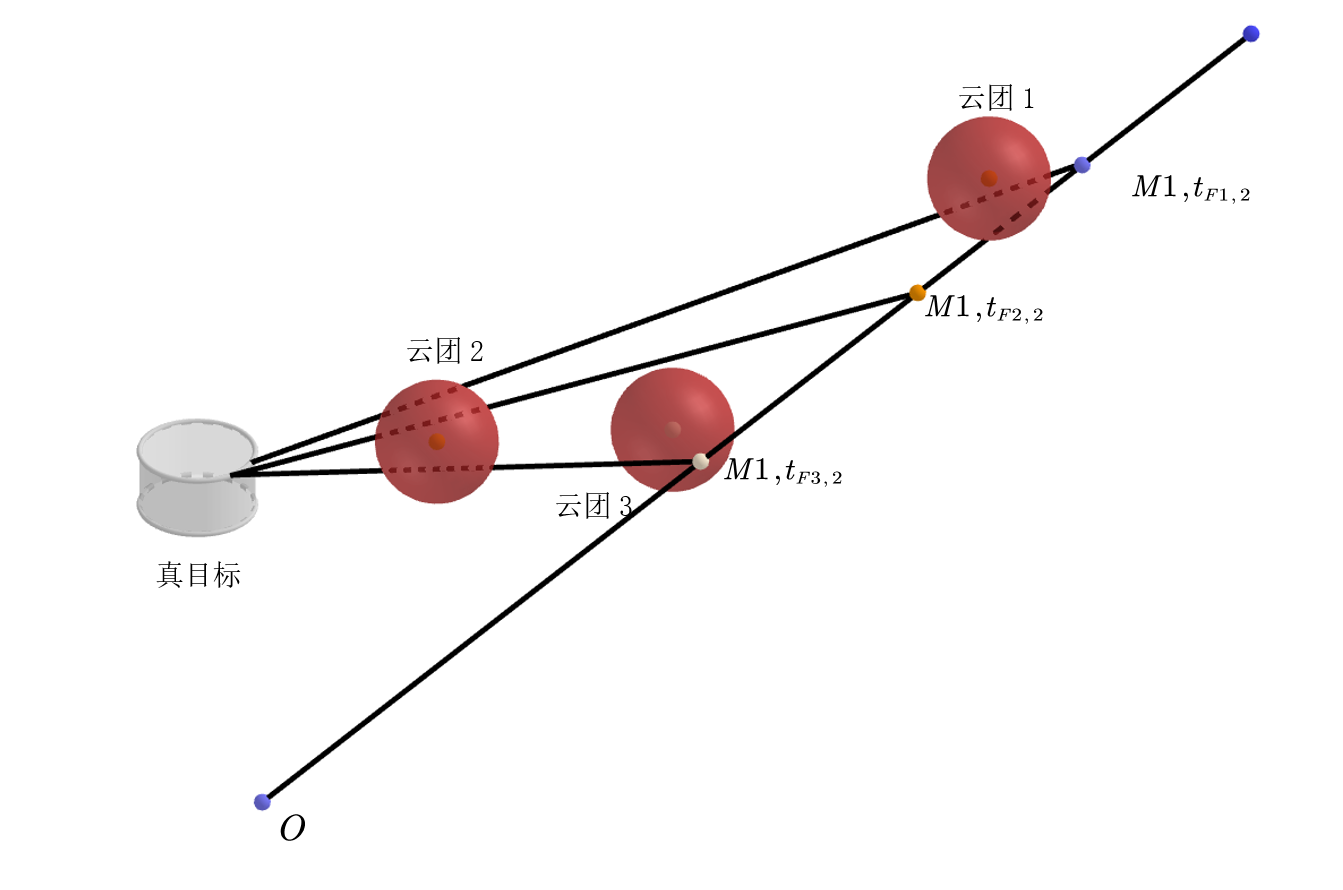
\includegraphics[scale=0.5]{图三.png}
\caption{}
\label{图3}
\end{figure}



\end{document}